\scanpage{70}\mspage{69}
J'en viens à la rel d'ordre $\preceq$ (subdivision), de nature \unsure{très|trs} différente. Il n'y aura pas de plus petit (ni de plus grand) élément, pas de $\mathrm{Sup}$ de deux \deleted{\unsure{éléments|élémen}} figures \inserted{$F',F''\,\unsure{\preceq|\deleted{\preceq}}-$} toujours (i.e. Subdivisions d'une = figure $F$, mais parfois un $\inf$.

On dit que deux subdivision $F',F'''$ de $F$ sont \uline{comp\deleted{\unsure{ati|atib}}\unsure{ara|ati|ata}bles} \deleted{\unsure{quand et|on dit} que \unsure{seul|sub}} (je ne dirai pas ``compatibles'', vu que le terme est déjà pris) si elles admettent une subdivision commune.

% R3-DIAGRAM: the right-hand F is almost level with the upper F'.
% The upper-right relation has an extra upper arm; the interpretation as an older deleted relation is uncertain.
\diagram{\begin{tikzcd}[ampersand replacement=\&,row sep=0.1em,column sep=0.45em]
\& F' \arrow[r,phantom,"{\scriptstyle\unsure{\preceq|\deleted{\leq}\preceq|\deleted{\prec}\preceq}}" description] \& F \\
F''' \arrow[ur,phantom,"\scriptstyle\preceq" description,sloped] \arrow[dr,phantom,"\scriptstyle\preceq" description,sloped] \& \& \\
\& F'' \arrow[uur,phantom,"\scriptstyle\preceq" description,sloped] \&
\end{tikzcd}}
% slanted
\margin{On sera amené à renforcer encore cette condition sur les contrées modérées !}

On dit que la \uuline{\unsure{contrée|contrie}} est \uuline{modérée} si deux subdivisions \unsure{\deleted{d'}d'une|d'une|d'un} = $F$ sont toujours comparables. \deleted{Dans le cas qui vient,}
% R3-ON-A-POINTS: two distinct low points fall slightly to the right.
\figure{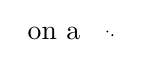
\begin{tikzpicture}[x=1em,y=1em,baseline=(ona.base)]
\node[anchor=base west,inner sep=0pt] (ona) at (0,0) {\deleted{on a}};
\fill (2.9,0.29) circle[radius=0.035];
\fill (3.08,0.16) circle[radius=0.04];
\end{tikzpicture}}

% The cancelled C5 stands at the left, below the opening Je... line.
\margin{\deleted{\uline{C5}}}
Je ne saurais donner aucune propriété particulière de $\preceq$ \deleted{tout} seul. Les propriétés que j'ai en vue concernent \unsure{ses|les} relations avec $\leq$.

% slanted
\margin{\unsure{Reporter|reporter} après C6, $C7_0$ ces axiomes de \uline{disjonction}}
% R3-C5-BARS: the two separate vertical rules stand beside the lower three lines of the axiom.
\figure{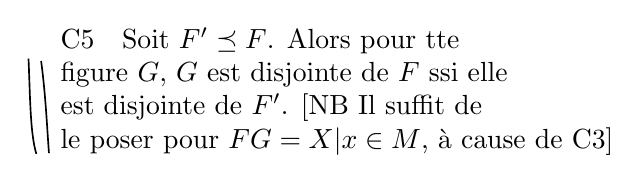
\begin{tikzpicture}[x=1cm,y=1cm]
\draw[line width=0.6pt] (0,-0.40) .. controls (0.02,-0.84) and (0.02,-1.36) .. (0.10,-1.61);
\draw[line width=0.6pt] (0.16,-0.43) .. controls (0.22,-0.87) and (0.24,-1.36) .. (0.26,-1.60);
\node[anchor=north west,inner sep=0pt,align=left] at (0.40,0) {\uline{C5}\quad Soit $F'\preceq F$. Alors pour tte\\
figure $G$, $G$ est disjointe de $F$ ssi elle\\
est disjointe de $F'$. [\uline{NB} Il suffit de\\
le poser pour $\deleted{\unsure{F}}G=\unsure{X|x}\in M$, à cause de C3]};
\end{tikzpicture}}
